\documentclass{beamer}
\usepackage[czech]{babel}
\usepackage[utf8]{inputenc}
\usetheme{Boadilla}
\usecolortheme{crane}
\title[Prezentace do IFJ a IAL]{Prezentace projektu do předmětů IFJ a IAL}
\author{Lukáš Brabec, Radka Mokrá, Aleš Dujíček, Jan Sedlák}
\begin{document}
\begin{frame}
  \maketitle
\end{frame}
\section{Popis projektu}
\begin{frame}{Hovadiny}
  Příliš žluťoučký kůň úpěl dábelské ódy.
  \begin{itemize}
    \item Beamer is a wonderful class
    \item One can make animations
    \item One uses the \textbf{pause} command, for example
    \item in order to bring in important ideas
  \end{itemize}
\end{frame}

\begin{frame}{Obrázek}
    \begin{figure}
        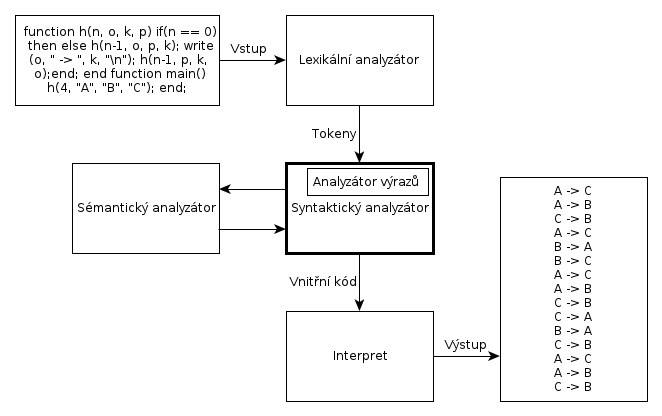
\includegraphics[scale=0.45]{schema.png}
        \caption{Schéma kompilátoru}
    \end{figure}
\end{frame}

\end{document}
